\chapter{系统设计}

\newcommand{\chapterfourplaceholder}[1]{%
\begin{samepage}
\begin{center}
\fbox{\parbox[c][4.2cm][c]{0.82\textwidth}{\centering #1（此处插入）}}
\end{center}
\begin{center}
#1（此处插入）
\end{center}
\end{samepage}
}

\section{系统总体设计}

系统的设计重点在保证实时通信能力基础上，整合技术问答、消息检索和知识沉淀等增强功能。这要求明确前后端分工，协调实时与常规业务链路，并统一消息记录和模型数据的存储体系。

\subsection{系统架构设计}

本系统采用前后端分离架构。前端基于 Vue 3，结合 Vite、Pinia 和 Vue Router 完成界面渲染与状态管理；后端运行于 Node.js 环境，通过 Express 提供 RESTful 接口，并由 Socket.IO 维持实时双向通信。这样的分层将界面逻辑与业务处理分离，便于后续维护与功能扩展\cite{vueguide2026,piniadocs2026,expressdocs2026,socketiodocs2026}。

前端主要由登录注册页、主聊天区和收藏浏览页构成，主窗口采用左侧导航、中间列表、右侧详情的三栏布局，移动端再根据小屏场景重新组织内容。状态由 Pinia 管理，HTTP 请求统一通过 Axios 封装；后端按认证、房间调度、消息收藏和 AI 服务等职责拆分模块，MongoDB 配合 Mongoose 完成数据持久化，AI 问答链路再结合向量检索组织上下文。整体分层见图~\ref{fig:4-1}。

\enlargethispage{2\baselineskip}
\begin{figure}[H]
\centering
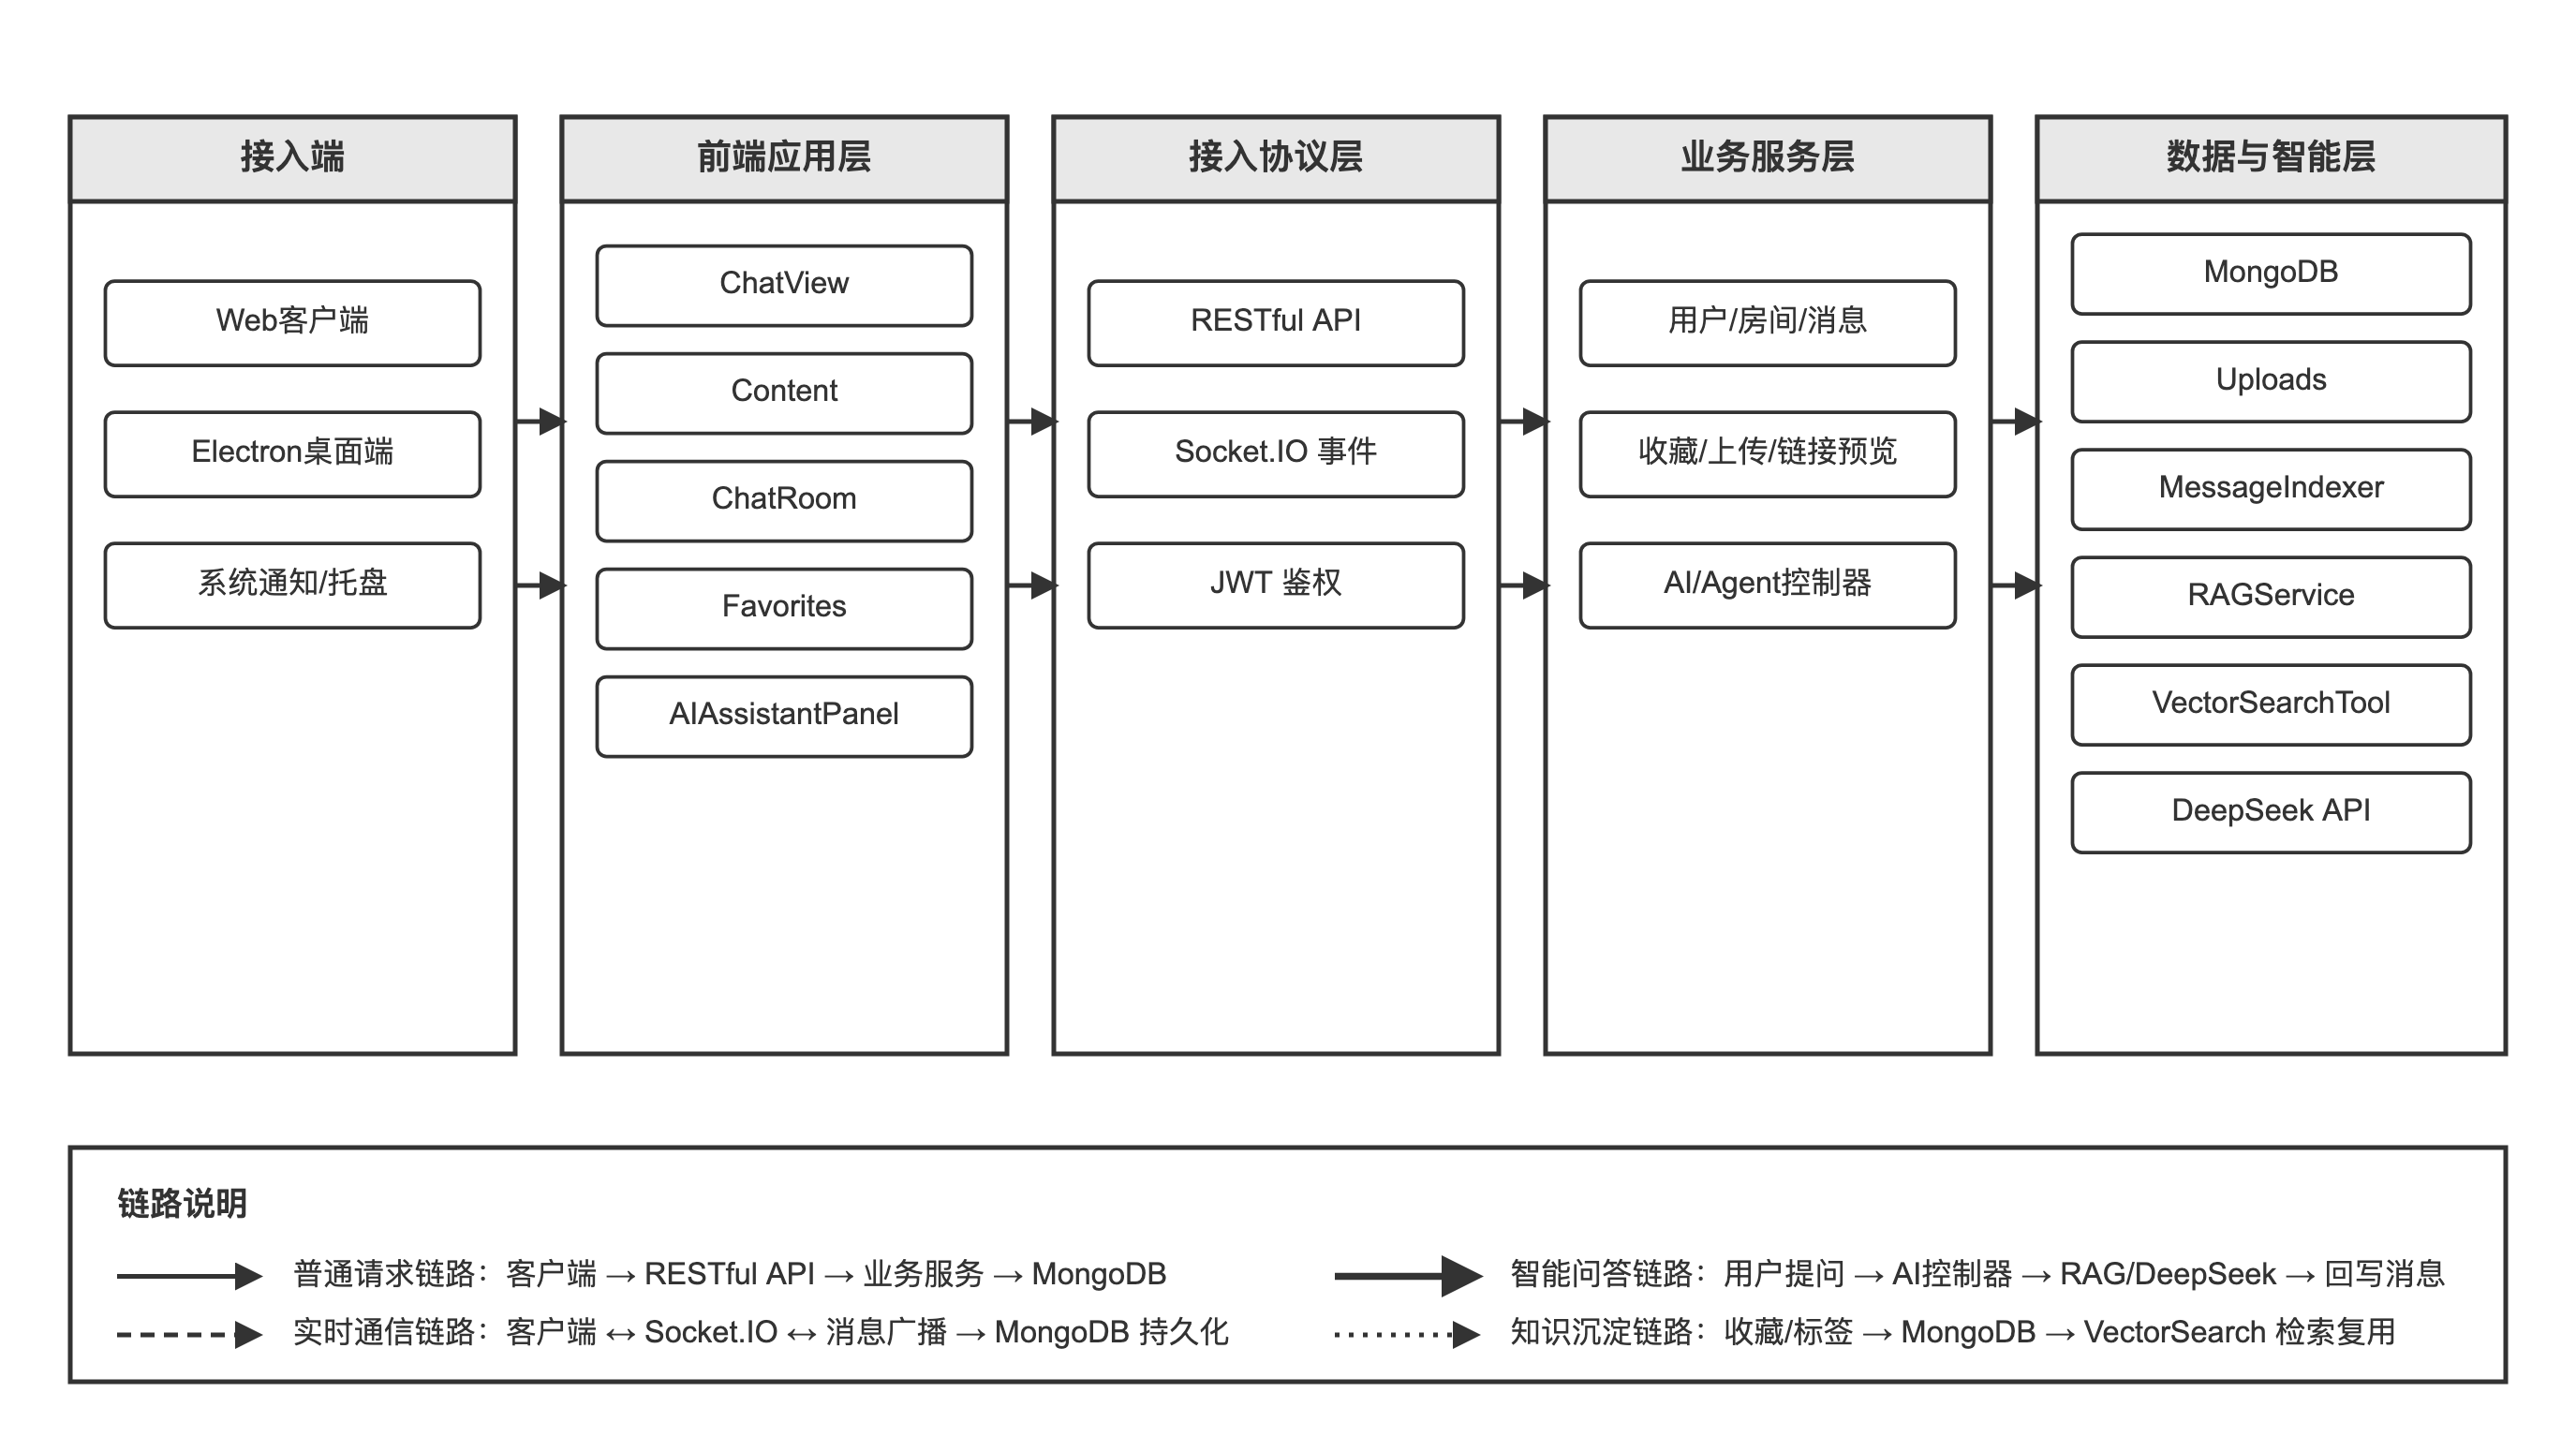
\includegraphics[width=0.82\textwidth,height=0.30\textheight,keepaspectratio]{img/图4_1.png}
\caption{系统架构图}
\label{fig:4-1}
\end{figure}

\FloatBarrier

\subsection{系统总体流程设计}

系统整体运行流程可分为身份认证、会话接入、消息收发、AI 辅助和结果沉淀五个阶段。用户通过邮箱密码或 OAuth2 完成登录后获取 JWT 令牌，再进入指定会话或聊天室发起请求与实时交互。

文本消息和各类附件先由 Express 完成校验与存储，再通过 Socket.IO 同步给相关在线用户。对于聊天室中的技术问题，用户可以调用 AI 助手生成回答，系统会结合当前上下文和检索结果组织提示信息。讨论结束后，用户还可以将摘要或关键代码收藏保存，形成后续复用的资料积累，如图~\ref{fig:4-2}。

\begin{figure}[H]
\centering
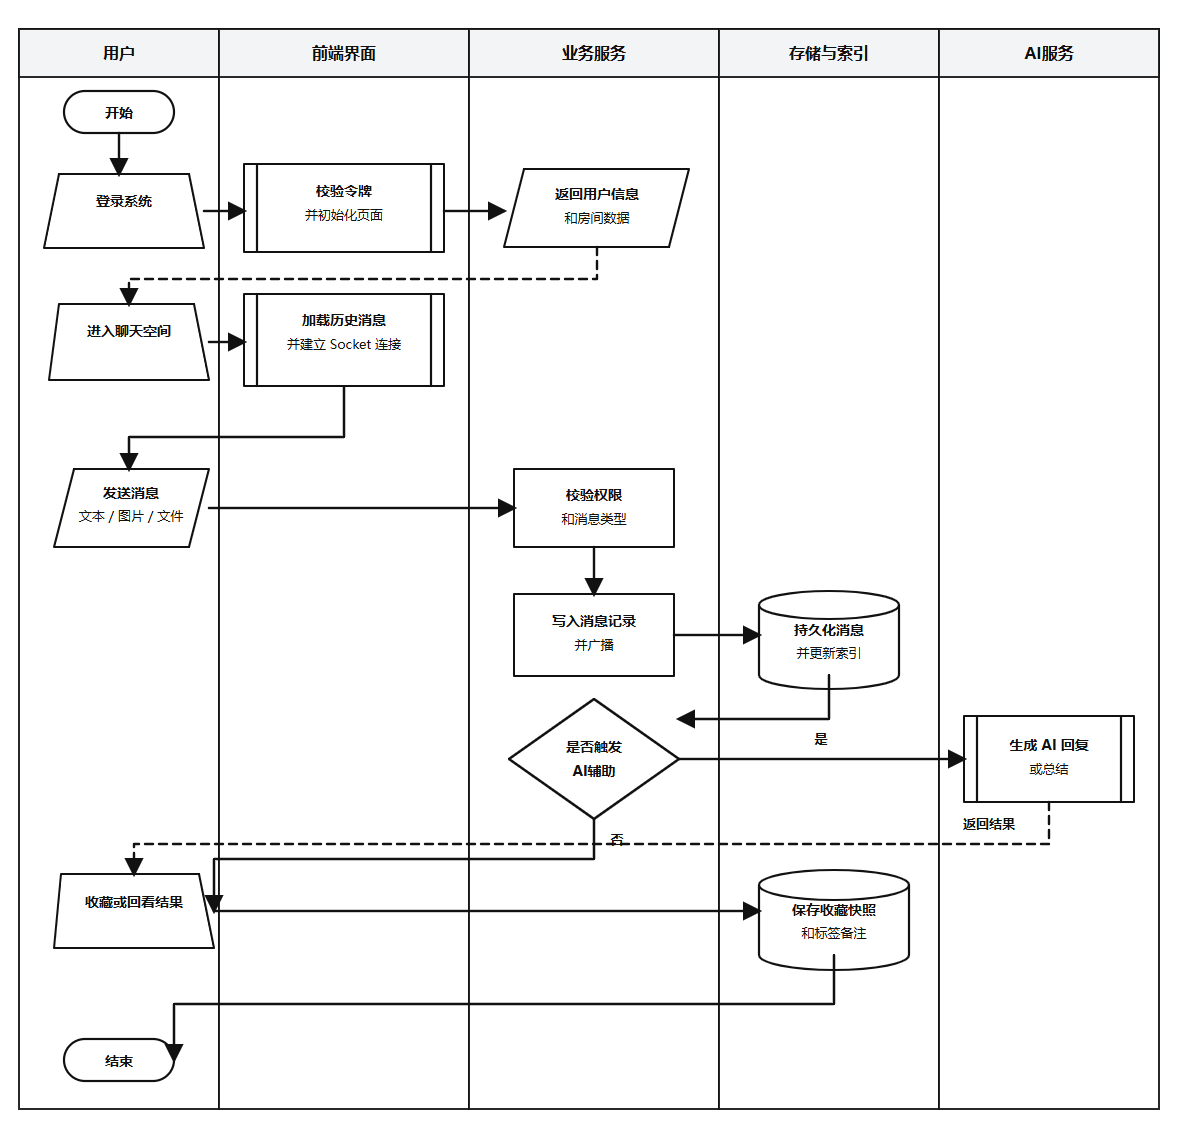
\includegraphics[width=0.94\textwidth,height=0.54\textheight,keepaspectratio]{img/图4_2.png}
\caption{系统总体流程图}
\label{fig:4-2}
\end{figure}

\subsection{系统功能结构设计}

依据业务目标，系统划分为五个核心子模块，包括用户管理、即时通讯、技术聊天室、AI 问答与总结，以及收藏归档。

这种划分便于明确各模块职责，也方便后续在不影响主要业务链路的前提下扩展语音功能或调整大模型接口，系统功能结构见图~\ref{fig:4-3}。

\begin{figure}[H]
\centering
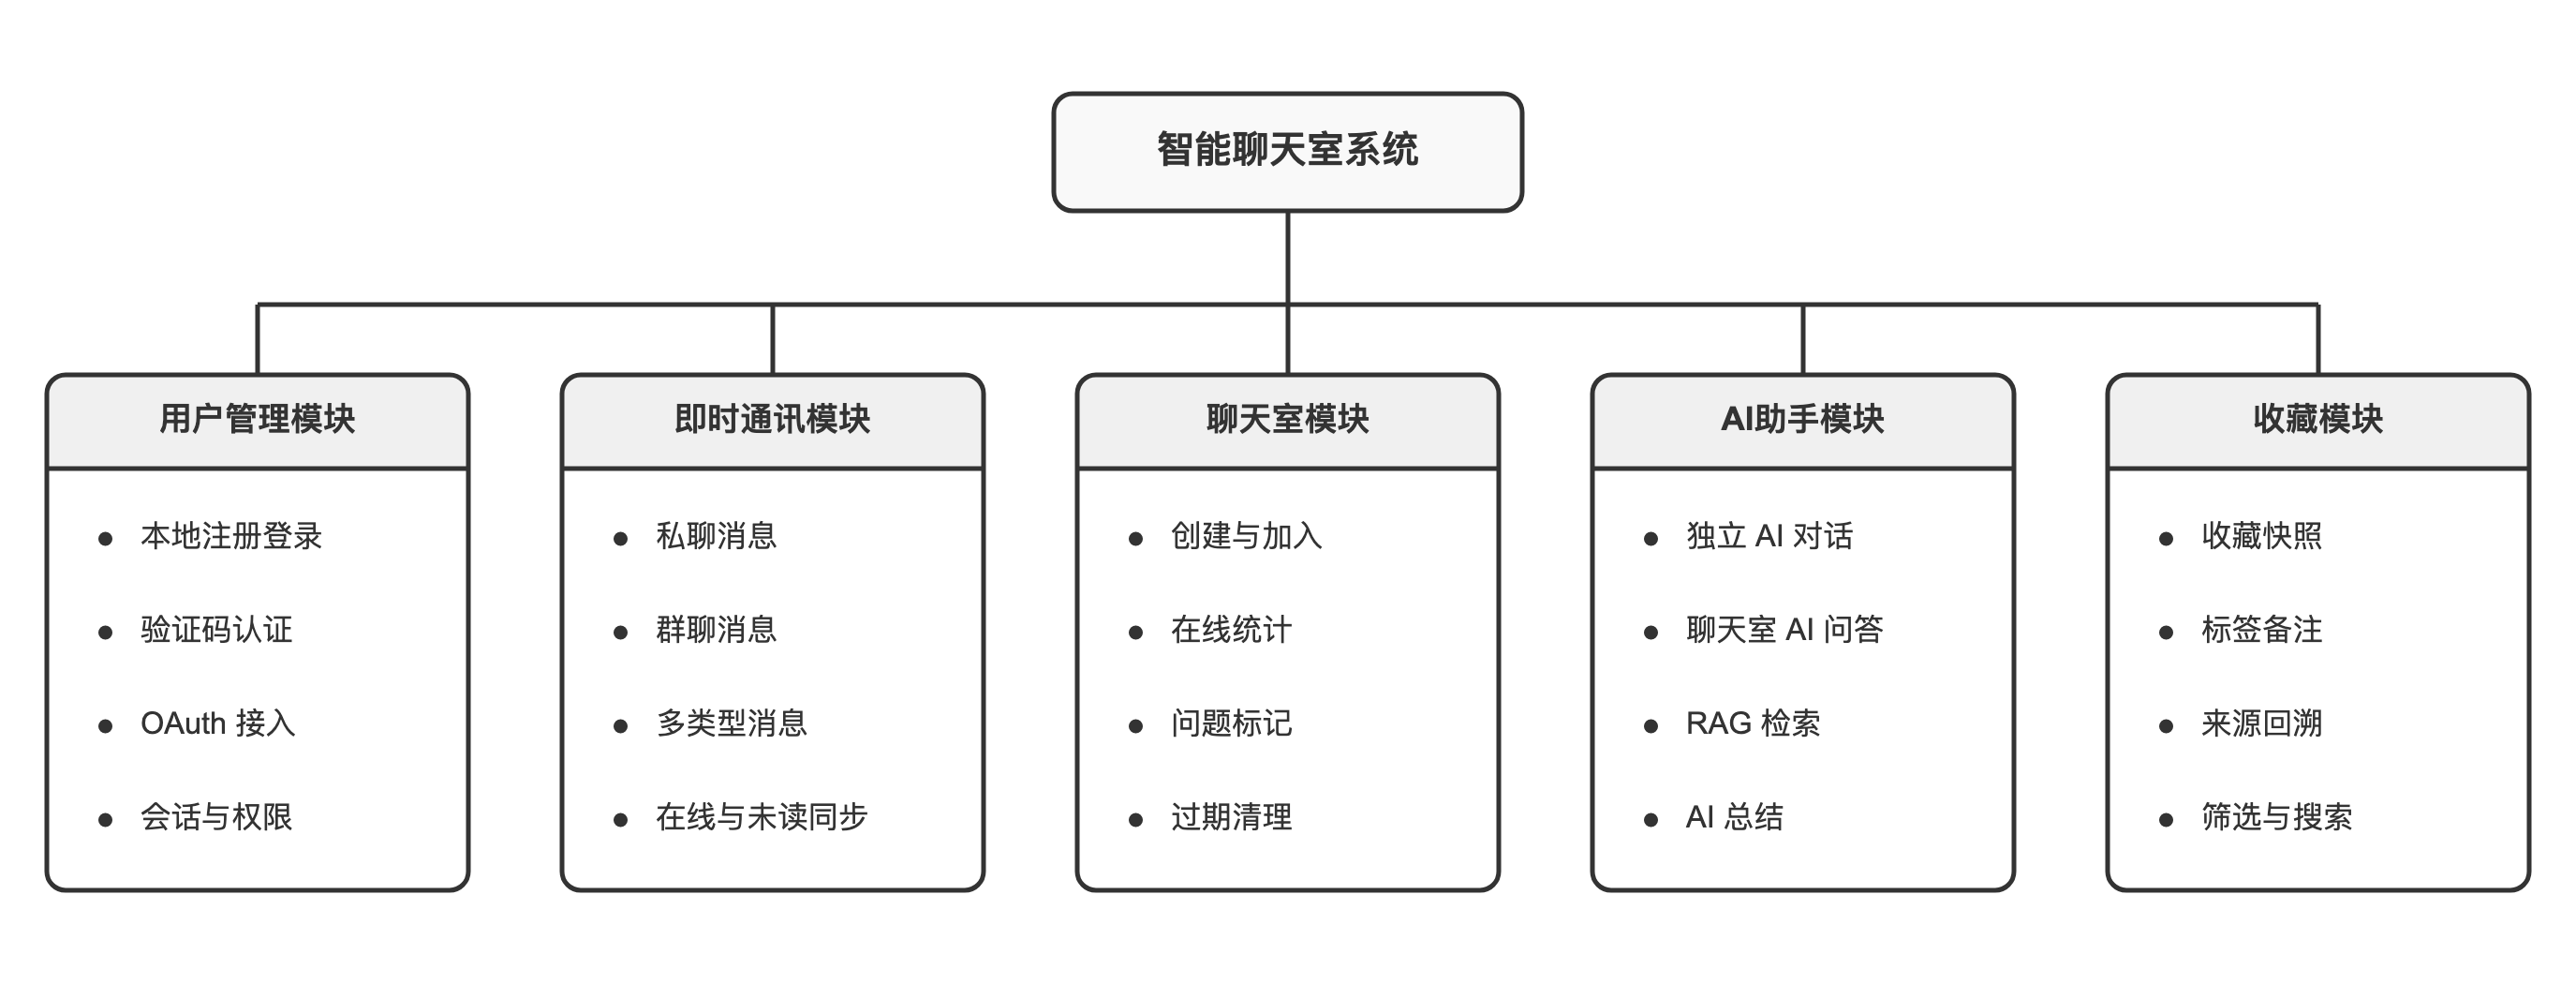
\includegraphics[width=0.95\textwidth, keepaspectratio]{img/图4_3.png}
\caption{系统功能结构图}
\label{fig:4-3}
\end{figure}

\section{功能模块设计}

在总体架构基础上，各功能模块继续按实际业务流程展开。

\subsection{用户管理模块}

用户管理模块负责注册、登录、身份校验和基础资料维护。本地登录流程包括邮箱查重、密码哈希存储和凭证校验，第三方登录则通过 Passport.js 对接 GitHub 和 Google 的 OAuth 授权流程，并在认证成功后返回系统凭证\cite{oauthcn2024,oauthbcp2025}。统一的用户标识会继续用于消息、收藏和聊天室等业务记录，模块内部运作序列如图~\ref{fig:4-4}所示。

\begin{figure}[H]
\centering
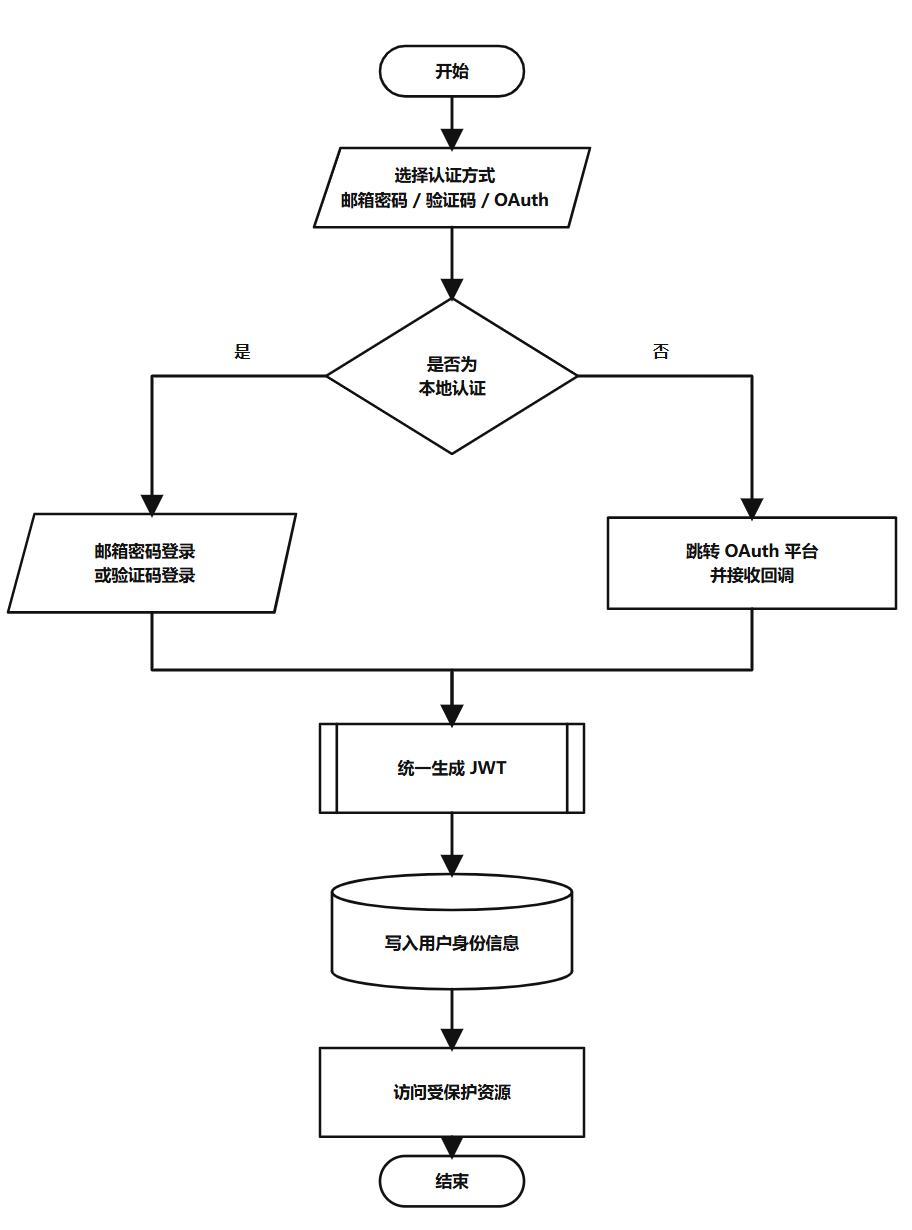
\includegraphics[width=0.94\textwidth,height=0.58\textheight,keepaspectratio]{img/图4_4.png}
\caption{用户模块流程图}
\label{fig:4-4}
\end{figure}

\subsection{即时通讯模块}

即时通讯模块负责私聊与群聊消息的收发和同步。系统将历史消息查询与持久化写入放在 HTTP 接口中，将实时推送交由 WebSocket 处理\cite{socketiodocs2026,imsecurity2024}。消息在写入私聊或群聊数据表后，再通过单播或房间广播分发给在线用户；文本、图片、文件等不同类型的消息也在这一层统一组织后返回前端，流程如图~\ref{fig:4-5}所示。

\begin{figure}[H]
\centering
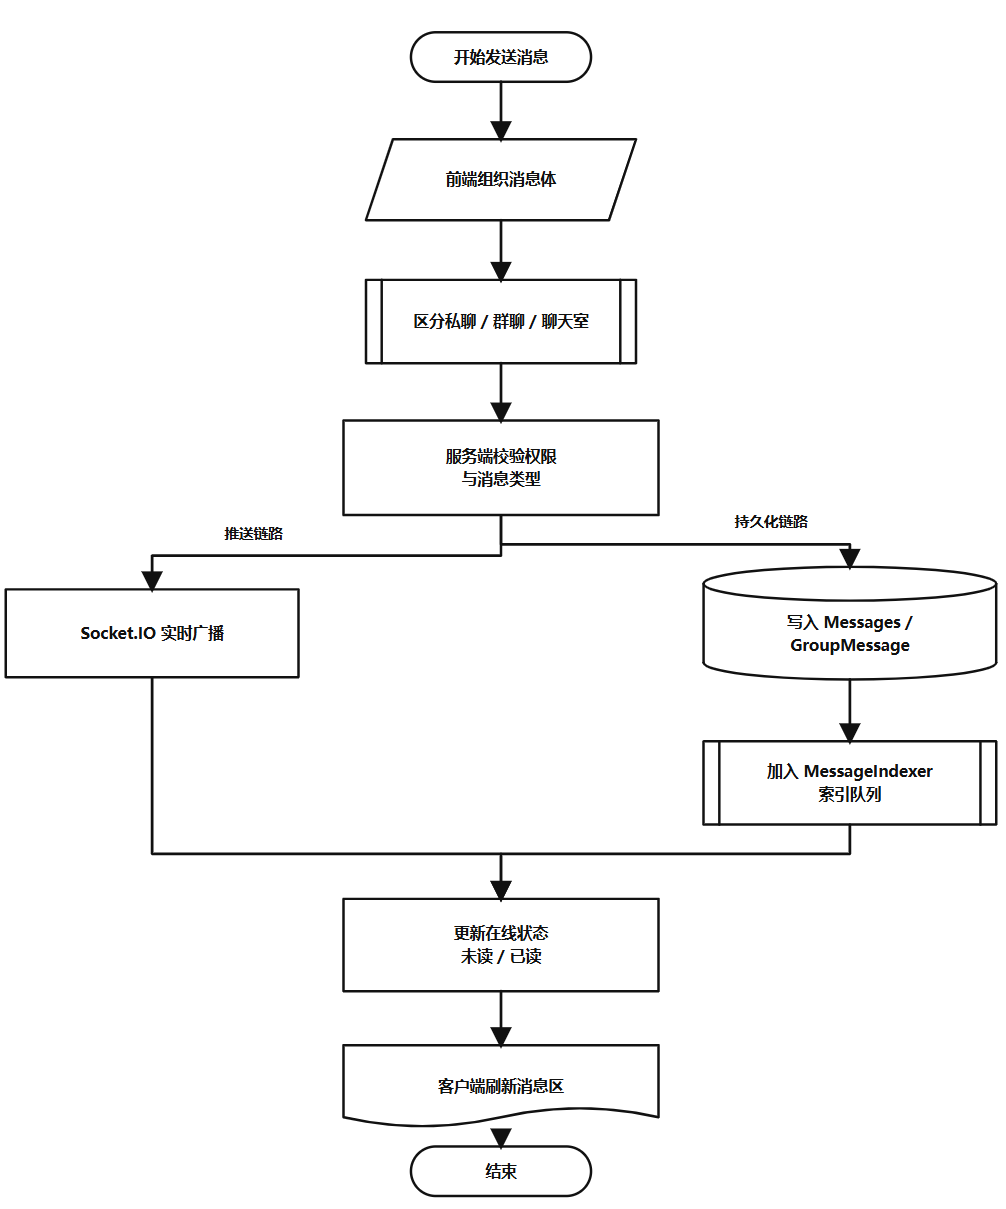
\includegraphics[width=0.94\textwidth,height=0.58\textheight,keepaspectratio]{img/图4_5.png}
\caption{即时通讯流程图}
\label{fig:4-5}
\end{figure}

\subsection{聊天室模块}

聊天室模块面向需要多人实时讨论的技术交流场景。该模块支持公开进入、口令校验或邀请加入等方式，并根据聊天室配置记录有效期与状态变化；当聊天室超期或被解散时，系统会停止新的交互请求并保留历史记录。整体流程如图~\ref{fig:4-6}所示。

\begin{figure}[H]
\centering
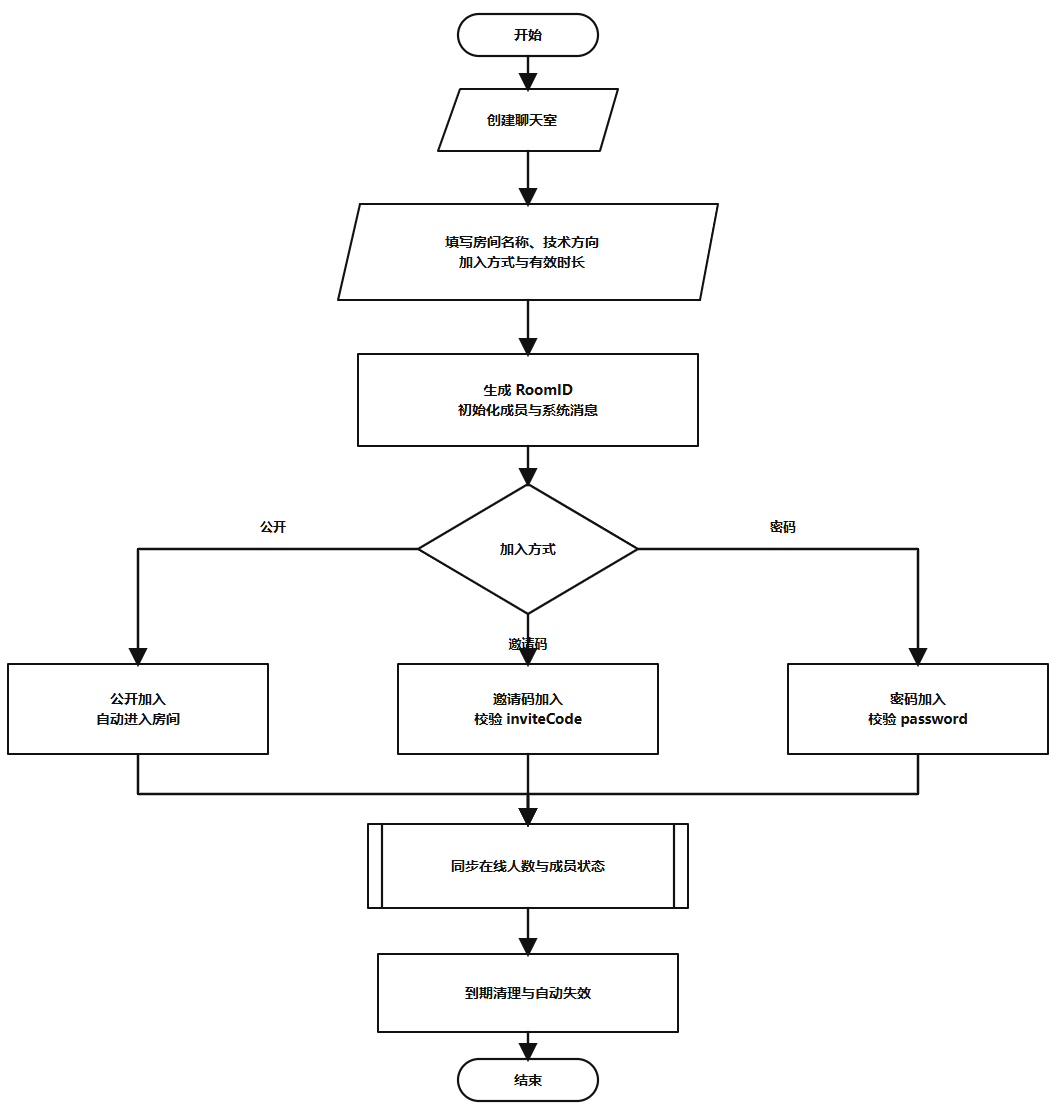
\includegraphics[width=0.94\textwidth,height=0.54\textheight,keepaspectratio]{img/图4_6.png}
\caption{聊天室流程图}
\label{fig:4-6}
\end{figure}

\subsection{AI助手智能问答模块}

AI 助手模块用于在现有聊天链路上提供问答、解释和总结能力。系统在请求模型前会先结合最近消息与检索结果组织上下文，再发起生成请求；返回阶段采用流式输出，并通过 WebSocket 将增量内容同步给房间内其他成员，从而降低等待时长。具体数据组织见图~\ref{fig:4-7}。

\begin{figure}[H]
\centering
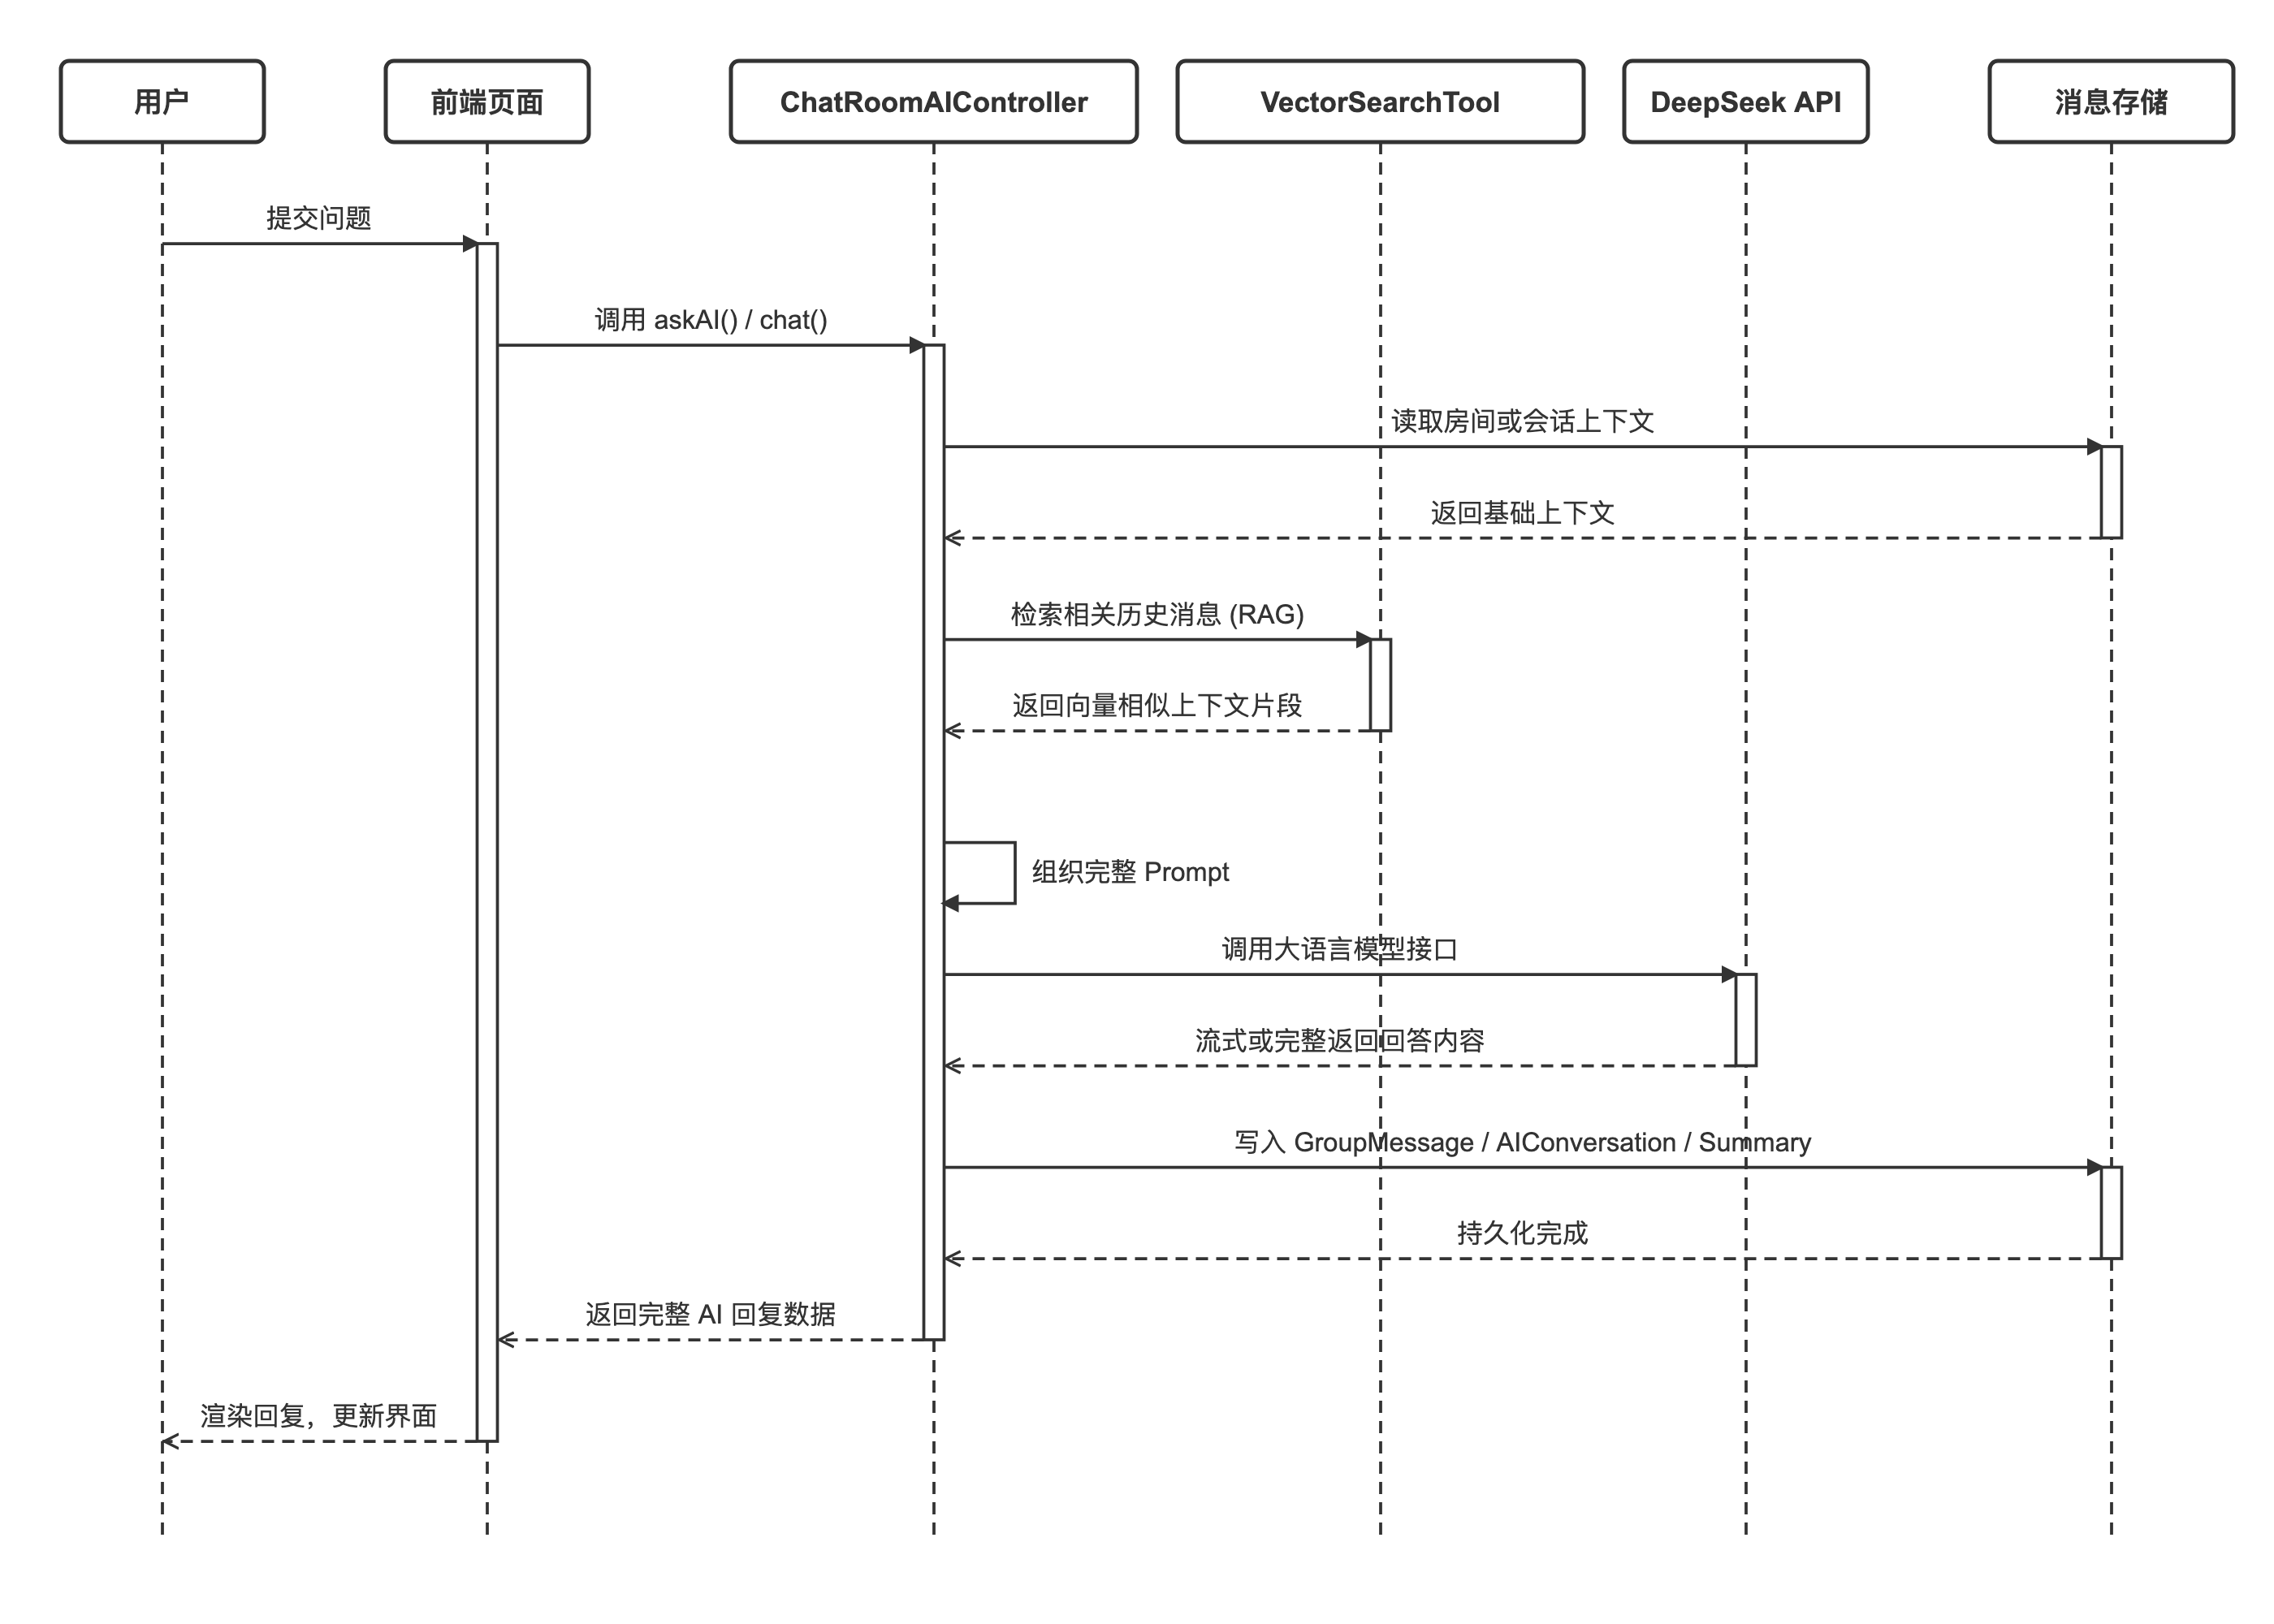
\includegraphics[width=0.94\textwidth,height=0.42\textheight,keepaspectratio]{img/图4_7.png}
\caption{AI助手智能问答模块时序图}
\label{fig:4-7}
\end{figure}

\subsection{收藏模块}

收藏模块用于保存讨论过程中的重要内容。系统在收藏时不仅记录消息标识，还会同步保存消息正文、附件信息和发送者等必要上下文，以便后续独立查看和回溯。用户还可以为收藏内容补充标签和备注，便于检索与整理，交互流程如图~\ref{fig:4-8}。

\begin{figure}[H]
\centering
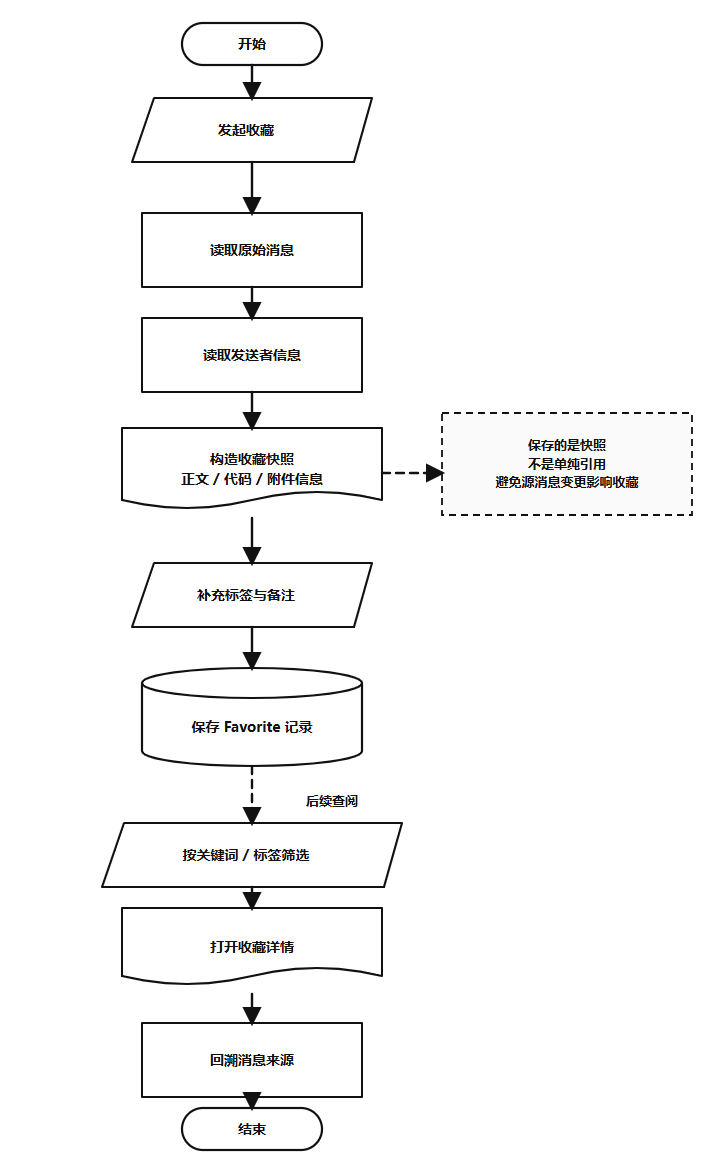
\includegraphics[width=0.94\textwidth,height=0.60\textheight,keepaspectratio]{img/图4_8.png}
\caption{收藏流程图}
\label{fig:4-8}
\end{figure}

\section{界面设计}

界面设计围绕消息阅读、输入操作和状态切换展开，重点保证长时间使用时的信息清晰度与操作连续性。

\subsection{登录与注册界面}
登录与注册界面采用卡片式切换结构，在同一页面中完成登录、注册和 OAuth 登录入口的展示。界面保留必要的表单项和状态提示，减少干扰信息，面板构成见图~\ref{fig:4-9}。

\begin{figure}[H]
\centering
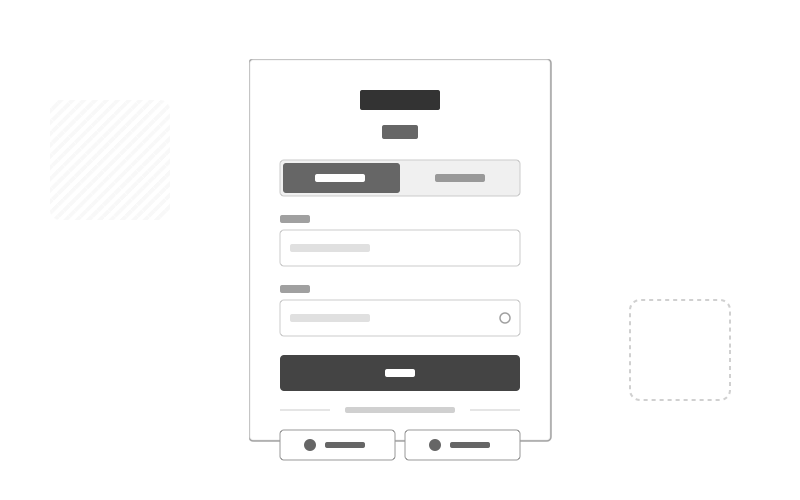
\includegraphics[width=0.88\textwidth,height=0.36\textheight,keepaspectratio]{img/图4_9.png}
\caption{登录与注册界面结构图}
\label{fig:4-9}
\end{figure}

\subsection{主聊天业务界面}
主聊天界面采用左侧导航、中间会话列表、右侧消息详情的三栏布局。该布局能够同时呈现会话切换、消息浏览和当前聊天内容，便于在代码片段、文件和普通文本之间快速切换\cite{vueguide2026,electrondocs2026}，如图~\ref{fig:4-10}所示。

\begin{figure}[H]
\centering
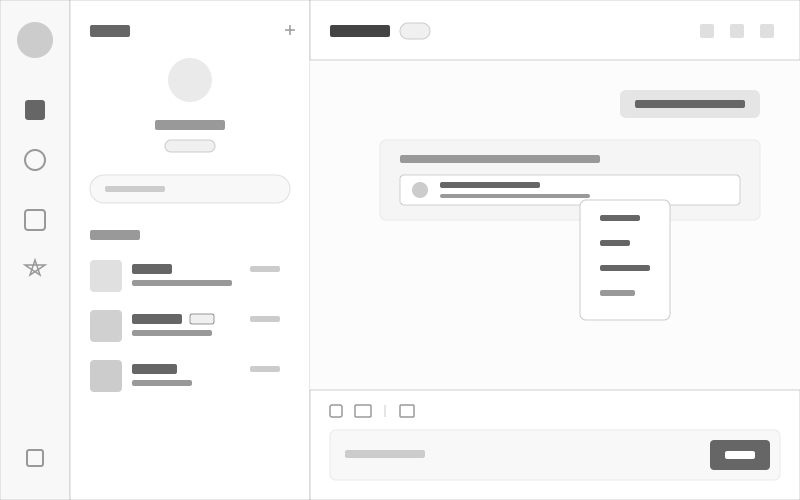
\includegraphics[width=0.88\textwidth,height=0.36\textheight,keepaspectratio]{img/图4_10.png}
\caption{主聊天界面结构图}
\label{fig:4-10}
\end{figure}

\subsection{沉浸式技术聊天室界面}
技术聊天室界面在主聊天布局基础上增加了倒计时、问题状态控制和代码输入辅助等元素，用于突出专题讨论场景。这样可以在多人协作时保持讨论主题集中，并方便用户围绕问题、回答和代码片段进行连续交流，见图~\ref{fig:4-11}。

\begin{figure}[H]
\centering
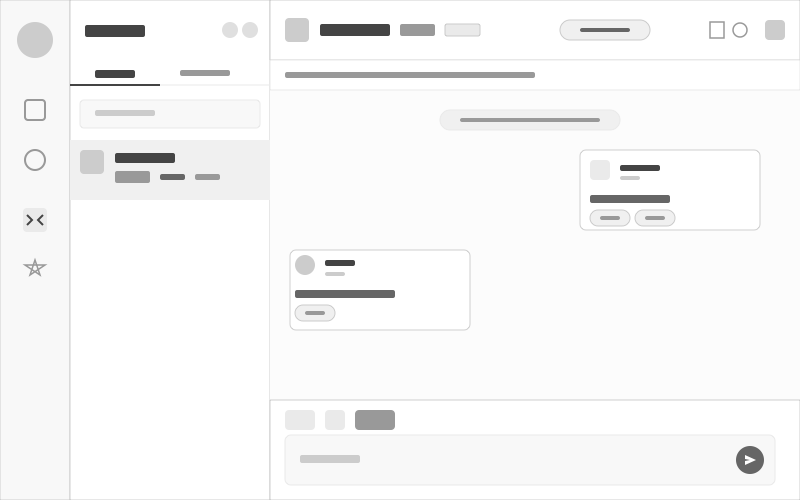
\includegraphics[width=0.88\textwidth,height=0.36\textheight,keepaspectratio]{img/图4_11.png}
\caption{聊天室界面结构图}
\label{fig:4-11}
\end{figure}

\section{数据库设计}

\subsection{E-R图设计}
系统选用 MongoDB 存储用户、房间、消息、收藏和 AI 相关数据，以适应消息类型多样、字段结构变化较快的业务特点。E-R 图以用户、聊天室和消息记录为核心，反映了收藏、AI 对话和总结等数据之间的关联关系，如图~\ref{fig:4-12}所示。

\begin{figure}[H]
\centering
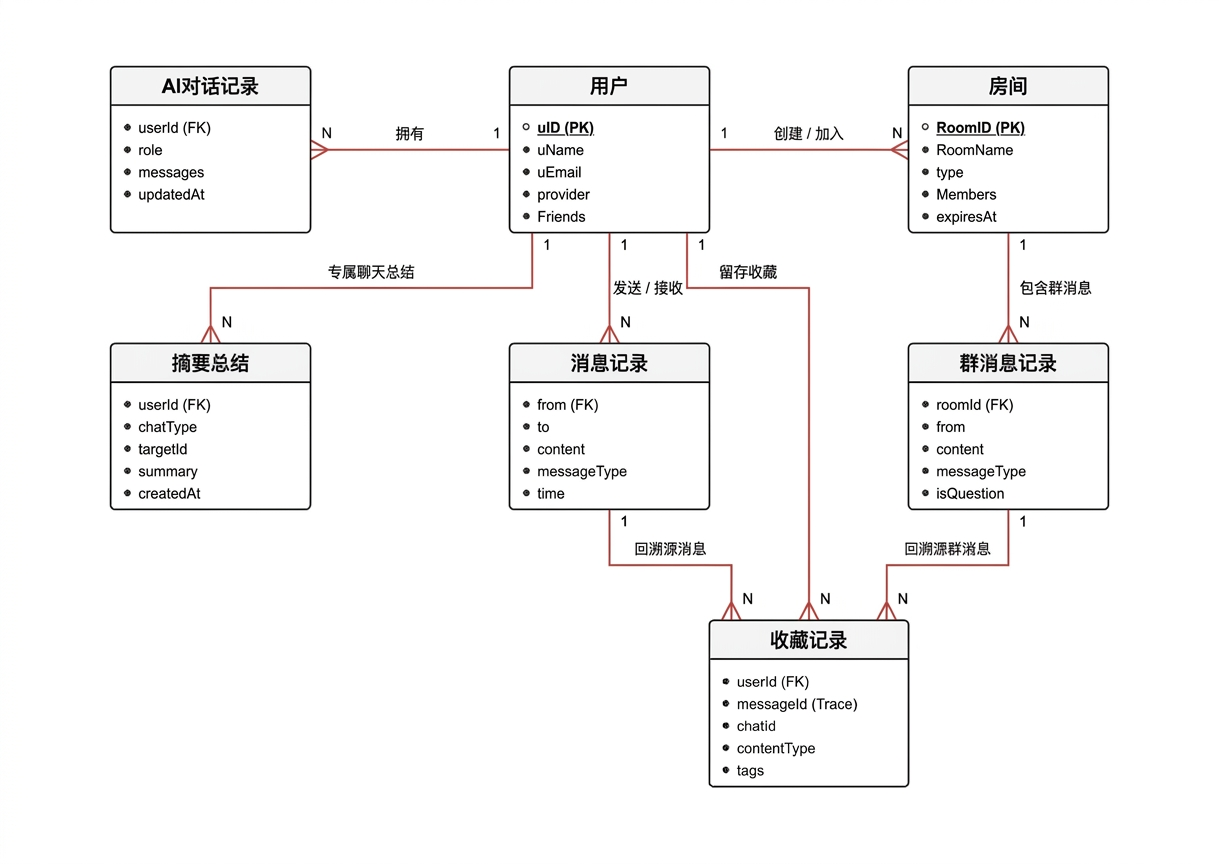
\includegraphics[width=0.88\textwidth,height=0.36\textheight,keepaspectratio]{img/图4_12.png}
\caption{系统数据库E-R图}
\label{fig:4-12}
\end{figure}

\subsection{数据库逻辑结构设计}

数据库逻辑结构设计需要同时考虑消息写入频率、历史查询和扩展字段等需求。基于 MongoDB 的文档模型，系统将核心业务数据拆分为 7 个主要集合，其结构说明如下\cite{mongodbdocs2026}。

\subsubsection{用户表设计}
用户表记录系统认证和身份展示所需的基础信息，如表~\ref{tab:4-1}所示。

\begin{table}[!htbp]
\centering
\caption{用户表结构}
\label{tab:4-1}
\small
\renewcommand{\arraystretch}{1.15}
\setlength{\tabcolsep}{0.6ex}
\begin{tabular}{M{0.17\textwidth}M{0.08\textwidth}M{0.13\textwidth}M{0.10\textwidth}p{0.34\textwidth}}
\toprule
\textbf{字段名} & \textbf{主键} & \textbf{数据类型} & \textbf{是否为空} & \textbf{说明} \\
\midrule
\_id & 是 & ObjectId & 否 & MongoDB 主键 \\
uID & 否 & String & 否 & 业务身份标识编码 \\
uName & 否 & String & 否 & 用户称呼展示 \\
uEmail & 否 & String & 否 & 登录邮箱地址 \\
Password & 否 & String & 是 & 密码哈希值，OAuth 用户可为空 \\
uAvatar & 否 & String & 否 & 用户头像地址 \\
Friends & 否 & Object[] & 是 & 好友列表 \\
googleId / githubId & 否 & String & 是 & 第三方平台用户标识 \\
provider & 否 & String & 否 & 登录来源 \\
\bottomrule
\end{tabular}
\end{table}

\subsubsection{聊天室表设计}
聊天室表用于保存房间基本信息、成员配置和加入方式等内容，如表~\ref{tab:4-2}所示。

\begin{table}[!htbp]
\centering
\caption{聊天室表结构}
\label{tab:4-2}
\small
\renewcommand{\arraystretch}{1.15}
\setlength{\tabcolsep}{0.6ex}
\begin{tabular}{M{0.17\textwidth}M{0.08\textwidth}M{0.13\textwidth}M{0.10\textwidth}p{0.34\textwidth}}
\toprule
\textbf{字段名} & \textbf{主键} & \textbf{数据类型} & \textbf{是否为空} & \textbf{说明} \\
\midrule
\_id & 是 & ObjectId & 否 & 文档主键 \\
\shortstack{RoomID\\RoomName} & 否 & String & 否 & 聊天室编号与名称 \\
\shortstack{Creator\\Admins} & 否 & String[] & 是 & 创建者与管理员列表 \\
Members & 否 & Object[] & 是 & 成员列表及加入时间 \\
type & 否 & String & 否 & 聊天室类型 \\
techDirection & 否 & String & 是 & 技术方向标签 \\
joinType / inviteCode & 否 & String & 是 & 加入方式或邀请码 \\
expiresAt & 否 & Date & 是 & 到期时间 \\
\bottomrule
\end{tabular}
\end{table}

\subsubsection{私聊消息表设计}
私聊消息表用于保存一对一聊天记录及其状态信息，如表~\ref{tab:4-3}所示。

\begin{table}[!htbp]
\centering
\caption{私聊消息表结构}
\label{tab:4-3}
\small
\renewcommand{\arraystretch}{1.15}
\setlength{\tabcolsep}{0.6ex}
\begin{tabular}{M{0.17\textwidth}M{0.08\textwidth}M{0.13\textwidth}M{0.10\textwidth}p{0.34\textwidth}}
\toprule
\textbf{字段名} & \textbf{主键} & \textbf{数据类型} & \textbf{是否为空} & \textbf{说明} \\
\midrule
\_id & 是 & ObjectId & 否 & 文档主键 \\
\shortstack{from\\to} & 否 & String & 否 & 发送方与接收方 \\
time & 否 & Date & 否 & 发送时间 \\
\shortstack{content\\fileInfo} & 否 & Mixed & 是 & 消息内容或附件信息 \\
\shortstack{isRead\\readTime} & 否 & Mixed & 是 & 已读状态与已读时间 \\
\bottomrule
\end{tabular}
\end{table}

\subsubsection{群聊与聊天室消息表设计}
群聊与聊天室消息表用于保存多人会话中的消息内容及互动状态，如表~\ref{tab:4-4}所示。

\begin{table}[!htbp]
\centering
\caption{群聊与聊天室消息表结构}
\label{tab:4-4}
\small
\renewcommand{\arraystretch}{1.15}
\setlength{\tabcolsep}{0.6ex}
\begin{tabular}{M{0.17\textwidth}M{0.08\textwidth}M{0.13\textwidth}M{0.10\textwidth}p{0.34\textwidth}}
\toprule
\textbf{字段名} & \textbf{主键} & \textbf{数据类型} & \textbf{是否为空} & \textbf{说明} \\
\midrule
\shortstack{roomId\\fromName} & 否 & String & 否 & 房间编号与发送者名称 \\
\shortstack{content\\messageType}& 否 & String & 是 & 消息内容与消息类型 \\
\shortstack{codeInfo\\fileInfo} & 否 & Object & 是 & 代码块信息或附件信息 \\
\shortstack{isQuestion\\isSolution}& 否 & Boolean & 否 & 是否为问题或是否标记为解答 \\
\shortstack{reactions\\upvotes} & 否 & Object[] & 是 & 表情反馈与点赞信息 \\
\bottomrule
\end{tabular}
\end{table}

\subsubsection{收藏表设计}
收藏表用于保存用户收藏的消息及其附加说明，如表~\ref{tab:4-5}所示。

\begin{table}[!htbp]
\centering
\caption{收藏表结构}
\label{tab:4-5}
\small
\renewcommand{\arraystretch}{1.15}
\setlength{\tabcolsep}{0.6ex}
\begin{tabular}{M{0.17\textwidth}M{0.08\textwidth}M{0.13\textwidth}M{0.10\textwidth}p{0.34\textwidth}}
\toprule
\textbf{字段名} & \textbf{主键} & \textbf{数据类型} & \textbf{是否为空} & \textbf{说明} \\
\midrule
\shortstack{userId\\messageId} & 否 & String & 否 & 收藏用户与来源消息 \\
\shortstack{chatId\\contentType} & 否 & String & 否 & 所属会话与内容类型 \\
\shortstack{content\\codeInfo} & 否 & Mixed & 是 & 收藏正文与代码信息快照 \\
\shortstack{tags\\note} & 否 & Mixed & 是 & 自定义标签与备注 \\
\bottomrule
\end{tabular}
\end{table}

\subsubsection{AI对话表设计}
AI 对话表用于保存用户与 AI 助手之间的历史对话，如表~\ref{tab:4-6}所示。

\begin{table}[!htbp]
\centering
\caption{AI对话表结构}
\label{tab:4-6}
\small
\renewcommand{\arraystretch}{1.15}
\setlength{\tabcolsep}{0.6ex}
\begin{tabular}{M{0.17\textwidth}M{0.08\textwidth}M{0.13\textwidth}M{0.10\textwidth}p{0.34\textwidth}}
\toprule
\textbf{字段名} & \textbf{主键} & \textbf{数据类型} & \textbf{是否为空} & \textbf{说明} \\
\midrule
\shortstack{userId\\role} & 否 & String & 否 & 所属用户与角色类型 \\
rolePrompt & 否 & String & 是 & 角色提示词 \\
messages & 否 & Object[] & 是 & 对话消息列表 \\
\bottomrule
\end{tabular}
\end{table}

\subsubsection{聊天总结表设计}
聊天总结表用于保存会话的阶段总结结果及相关统计信息，如表~\ref{tab:4-7}所示。

\begin{table}[!htbp]
\centering
\caption{聊天总结表结构}
\label{tab:4-7}
\small
\renewcommand{\arraystretch}{1.15}
\setlength{\tabcolsep}{0.6ex}
\begin{tabular}{M{0.17\textwidth}M{0.08\textwidth}M{0.13\textwidth}M{0.10\textwidth}p{0.34\textwidth}}
\toprule
\textbf{字段名} & \textbf{主键} & \textbf{数据类型} & \textbf{是否为空} & \textbf{说明} \\
\midrule
\shortstack{targetId\\chatType} & 否 & String & 否 & 总结对象编号与会话类型 \\
summary & 否 & Object & 否 & 总结结果对象 \\
\shortstack{statistics\\msgCount} & 否 & Mixed & 是 & 统计信息与消息数量 \\
\bottomrule
\end{tabular}
\end{table}

\section{核心底层机制与部署拓扑设计}

\subsection{WebSocket 即时通信协作机理}

系统使用 WebSocket 处理消息实时分发和房间状态同步。服务端在消息写入或状态变更后向对应用户或房间广播事件，客户端接收事件后再更新消息列表、未读状态和界面显示，从而保证实时通信与持久化数据保持一致，具体机理如图~\ref{fig:4-13}所示。

\begin{figure}[H]
\centering
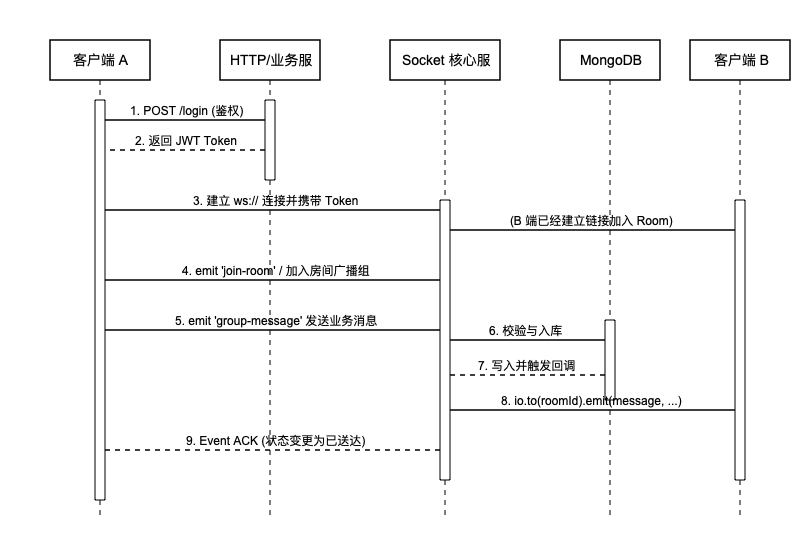
\includegraphics[width=0.94\textwidth,height=0.42\textheight,keepaspectratio]{img/图4_13.png}
\caption{Socket即时通信底层时序图}
\label{fig:4-13}
\end{figure}

\subsection{系统物理部署与网络拓扑架构}

在物理部署上，Nginx 负责统一接收外部请求并转发到 Express 与 Socket.IO 服务，MongoDB 用于保存用户、消息和收藏等业务数据，DeepSeek 模型服务负责处理需要生成能力的请求，整体网络拓扑如图~\ref{fig:4-14}所示。

\begin{figure}[H]
\centering
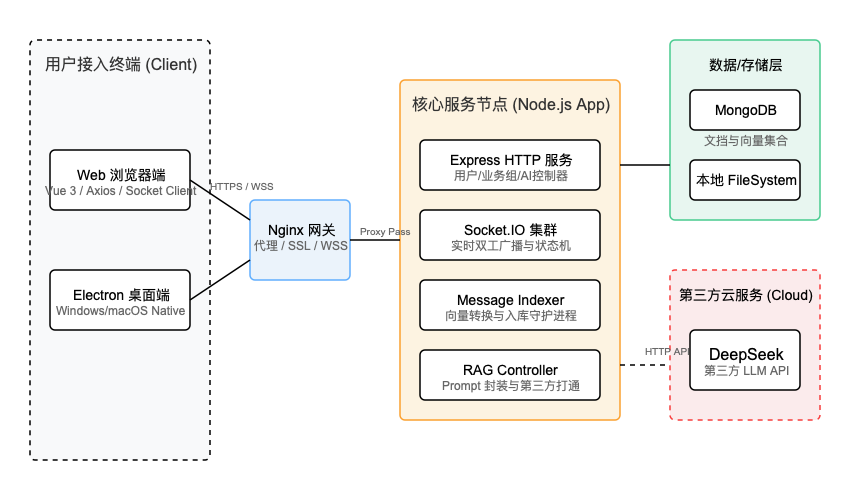
\includegraphics[width=0.90\textwidth, keepaspectratio]{img/图4_14.png}
\caption{系统物理部署与网络拓扑架构图}
\label{fig:4-14}
\end{figure}

从部署关系看，Web 端与桌面端共享同一套后端服务入口，实时通信、历史索引与 AI 能力围绕业务服务层统一组织。
